\section{Filtri}

Un riverbero artificiale, algoritmico, digitale, come quello proposto da \ms,
fonda tutta la sua architettura sull'idea di filtro, sulle relazioni tra filtri.

\subsection{Funzione di trasferimento}

La funzione di trasferimento è la trasformata della risposta all’impulso di un
sistema LTI (Linear Time-Invariant) e ne riassume le caratteristiche.

Si presenta nella seguente forma:

\begin{equation}
H(s)=\frac{\sum_{k=0}^K a_k s^k}{\sum_{n=0}^N a_n s^n}
\end{equation}

È definita tramite una funzione razionale fratta, ovvero una funzione costituita
dal rapporto di due polinomi. Ognuno dei due polinomi individua un’equazione
rispettivamente di $k$-mo e $n$-mo grado ovvero che ci saranno $k$ soluzioni
per il polinomio al numeratore ed $n$ soluzioni per il polinomio al denominatore.
Queste soluzioni saranno tutti i valori che rendono nulla la funzione:
quelle che azzerano il numeratore si dicono \textbf{zeri} $(-zk)$, quelle che
azzerano il denominatore si dicono \textbf{poli} $(-pn)$.

La forma fattorizzata della funzione di trasferimento è la seguente ed è
utilizzata per il tracciamento dei grafici di risposta in frequenza dei filtri
(detti diagrammi di bode)

\begin{equation}
H(s)=\frac{\prod_{k=1}^k (s+zk)}{\prod_{n=1}^n (s+pn)}
\end{equation}

Semplificando il tutto e ricollegandoci all’argomento principale, è necessario
comprendere che poli e zeri corrispondono alla frequenza di taglio del filtro
che la funzione di trasferimento rappresenta.

\subsection{Low-Pass}

Permette l’attenuazione delle frequenze superiori alla frequenza di taglio.
La sua funzione di trasferimento è la seguente

\begin{equation}
H(s)=\frac{1}{1+st}
\end{equation}

dove con $st$ indichiamo la frequenza di taglio.

\begin{figure}[h]
\centering
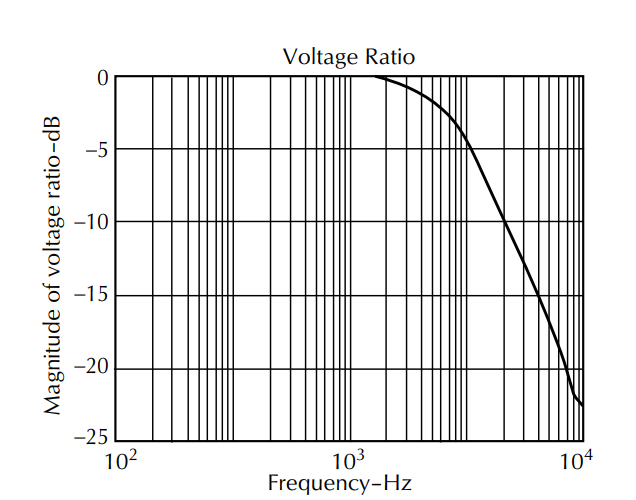
\includegraphics[width=0.80\textwidth]{lp}
\caption{Diagramma di Bode di un filtro passa basso \newline \scriptsize{ da D. Davis - Sound System Engineering - 2013}}
\label{fig:lp}
\end{figure}

\subsection{High-Pass}

Permette l’attenuazione delle frequenze inferiori alla frequenza di taglio.
La sua funzione di trasferimento è in figura \ref{fig:hp}

\begin{equation}
H(s)=\frac{st}{1+st}
\end{equation}

dove con $st$ indichiamo sempre la frequenza di taglio.
La risposta in frquenza ottenuta è la seguente

\begin{figure}[htp]
\centering
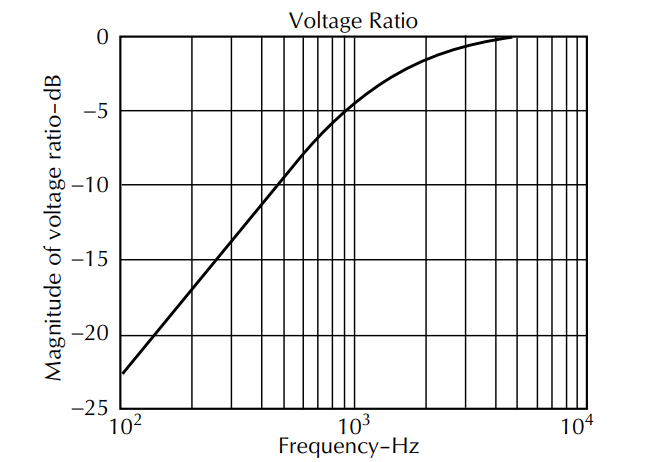
\includegraphics[width=0.80\textwidth]{hp}
\caption{Diagramma di Bode di un filtro passa alto}
\label{fig:hp}
\end{figure}

\subsection{Filtri Digitali}

Ttutto ciò che abbiamo visto fino a questo punto è puramente nel dominio
continuo. Possiamo dunque procedere all’implementazione di tali modelli
matematici in digitale. I filtri digitali utilizzano in larga scala algoritmi
ricorsivi aventi al loro interno moltiplicazioni e addizioni, per i quali gli
attuali strumenti informatici di cui disponiamo, sono ottimizzati. Definiamo
due macro categorie di filtri digitali ovvero i cosiddetti filtri \textbf{FIR}
e \textbf{IIR}.

\begin{itemize}
\item IIR: Infinite impulse response;
\item FIR: Finite impulse response.
\end{itemize}

Possiamo definire i filtri IIR come caratterizzati da una risposta all’impulso
unitario non limitata (parlando di numero di campioni) e un’ampiezza tendente
a zero. Questo rende i filtri IIR molto simili alla loro controparte analogica
(esistente nel tempo continuo). Per quanto riguarda la loro composizione
strutturale, notiamo generalmente una funzione di trasferimento costituita da
un rapporto polinomiale, con poli e zeri. È esclusa una situazione in cui siano
presenti soli zeri. Inoltre la costruzione di questi filtri prevede l’utilizzo
di sistemi di feedback, e per questo, è risaputo che queste strutture hanno un
comportamento instabile.

Parlando di filtri FIR, invece, possiamo affermare che la loro risposta
all’impulso unitario è composta da un numero finito di campioni e per questo
non associabili a nessun modello analogico.

A differenza dei filtri IIR, i filtri FIR, presentano una funzione di
trasferimento a soli zeri. Possedere una risposta all’impulso unitario limitata
comporta, inoltre, una stabilità nell'implementazione, ma di conseguenza una
necessità di maggiore potenza di calcolo.

%(Lindoro del Duca - Musica Digitale - pag 85)

\subsection{Delay}

Il \emph{Delay} è il ritardo temporale imposto ad una informazione in transito
(segnale). Il Delay può essere osservato soltanto se messo in relazione a se
stesso non ritardato.

Il delay è inoltre un componente chiave nella costruzione dei filtri digitali.

L’espressione che determina il comportamento del filtro è detta equazione
differenza e, in base al numero di elementi di ritardo presenti, possiamo
indicare l’ordine dell’equazione.

L’equazione differenza del primo ordine generale è definita secondo la seguente
equazione:

\begin{equation}
Y(z)=A_0*x(z) + A_1*z^{-1}*x(z) + B_1*z^{-1}*y(z)
\end{equation}

L’equazione è scritta nel dominio $z$, con $z$ detta frequenza complessa.
I valori di $z$ che rendono rispettivamente nullo numeratore e denominatore
vengono detti zeri e poli della funzione.

Tutte le equazioni differenza del primo ordine sono determinate dai
coefficienti $A_0,A_1,B_1$. È necessario considerare che un’equazione del primo
ordine può descrivere solo un filtro passa basso o passa alto avente
un’attenuazione di massimo 6 dB/ottava.

Partendo dall’equazione differenza, infine, possiamo ricavare la funzione di
trasferimento $H(z)$ avente la seguente forma:

\begin{equation}
H(z)=\frac{(A_0 + A_1 * z^{-1})} {(1-B_1 * z^{-1})}
\end{equation}

\lstinputlisting{Code/fir.dsp}

\begin{figure}[htp]
\centering
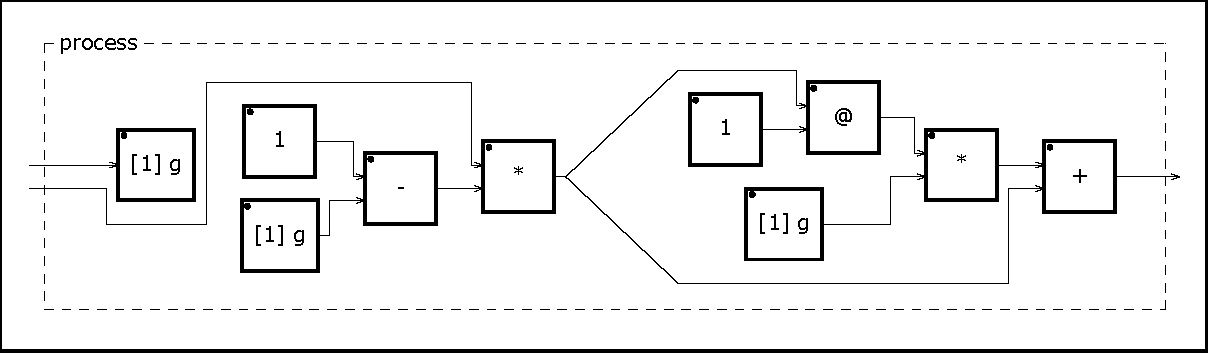
\includegraphics[width=0.80\textwidth]{Code/fir-svg/process.pdf}
\caption{Filtro \emph{FIR} con $g$ tra $0$ e $1$ il filtro è passa basso,
         con $g$ tra $0$ e $-1$ il filtro è passa alto.}
\label{fig:fir}
\end{figure}

\todo[inline]{tutto ciò che segue, dove analizzi filtri che poi non utilizzi nella
tesi non serve assolutamente a niente. puoi lasciare il filtro passa basso se lo
spieghi per gli usi che ne farai dopo nella riverberazione. }




% Alcune caratteristiche presenti nella maggior parte dei filtri sono:
%
% \begin{itemize}
% \item Banda Passante:
% Banda di frequenze che passa attraverso un filtro e che subisce una perdita di meno di 3 dB;
% \item Banda Stoppata:
% Banda di frequenze che passa attraverso un filtro e che subisce una perdita di 3 db o più;
% \item Frequenza di Taglio
% È la frequenza dove il filtro inizia ad eseguire modifiche al segnale, come abbattimenti o enfatizzazioni;
% \item Ordine:
% È una caratteristica definita dal numero di oggetti all’interno del filtro che concorrono al medesimo risultato, di solito inerenti a scopi di risposta in frequenza del filtro. Se tutti gli elementi sono eterogenei, per esempio passa basso o passa alto, l’attenuazione sarà di 6 db per ordine. Un filtro passa basso del quarto ordine avrà abbattimento di 24 db, ma un passa banda del medesimo ordine ne abbatterà soltanto 12.
% \end{itemize}
%
% \medskip
%
% \subsection{Categorie di filtri}
%
% In seguito a queste caratteristiche, passiamo ad eseguire brevi categorizzazioni di filtri in base alla loro componentistica e comportamenti.
%
% Una prima categorizzazione che possiamo eseguire, riguarda la presenza o meno, di componenti che amplificano il segnale. Parliamo di:
%
% \begin{itemize}
% \item Filtri Passivi:
% Sono filtri che non possiedono amplificatori di segnale, quindi il loro unico scopo è quello di attenuare ciò che li attraversa;
% \item Filtri Attivi:
% Al contrario, i filtri attivi hanno componenti che permettono l’amplificazione di determinate bande o dell’intero segnale, aggiungendo energia dove necessario.
% \end{itemize}
%
% Parliamo di \textbf{equalizzatore} per identificare un dispositivo il cui scopo è quello di sopperire a caratteristiche non gradite, riguardanti ampiezza, frequenza o fase, in modo tale da ricreare la risposta desiderata. Gli equalizzatori, per compiere ciò, sono costituiti da filtri, implementati per svolgere diversi tipi di modifiche.
%
%
% \section{Tipologie di filtro}
% Come detto in precedenza, i filtri si distinguono per via della loro architettura alla quale consegue un diverso comportamento. Ecco alcune tipologie di filtro, tra le più comuni:
%
%
% \subsection{Band-Pass}
% Permette il passaggio solo ad una determinata banda di frequenze.
% la sua funzione di trasferimento è la seguente
% \begin{equation}
% H(s)=\frac{(1+st_1)(1+st_4)}{(1+st_2)(1+st_3)}
% \end{equation}
% Considerando che $t_1>t_2>t3_>t_4$ e che il calcolo di poli e zeri risulta: $z_1=1/t_1$, $z_2=1/t_4$, $p1_=1/t_2$, $p_2=1/t_3$ \dots
%
% La risposta in frquenza ottenuta è in figura \ref{fig:bp}
% \begin{figure}[htp]
% \centering
% 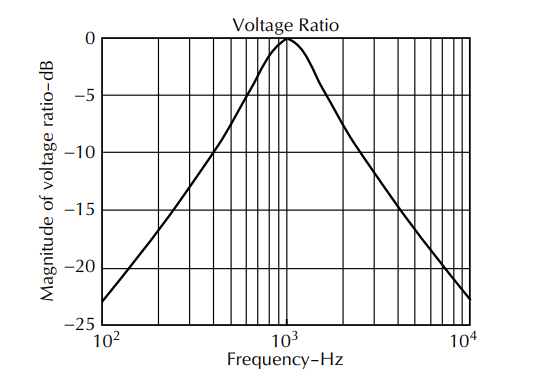
\includegraphics[width=%
% 0.50\textwidth]{bp}
% \caption{Diagramma di Bode di un filtro passa banda}
% \label{fig:bp}
% \end{figure}
